\chapter{Language systems and language strategies}

Although languages around the world exhibit an overwhelming variety in
the ways they describe colours, most of the research in the domain of
colour has focussed on the use of single colour terms to describe
colour. This approach has allowed psychologists to study the nature of
categories and it is now widely accepted that colour categories are organised around a
prototype which is the colour that represents a category best
\citep{rosch73natural}. The approach has also allowed to shed light
on the ongoing nature-nurture debate in which the question is to what
degree categories are innate and to what degree they are acquired
during the development of a child \citep{berlin69basic}.

In the field of artificial language evolution, researchers try to
model the origins and evolution of artificial languages in a
controlled environment. Within this field, the domain of colour has
been intensively studied. The focus on using a single colour term to
describe a colour sample has allowed researchers to formalise models
of how a population of artificial language users can form and
coordinate their own colour-related language system
\citep{steels05coordinating, belpaeme05explaining, belpaeme07language,
  puglisi08cultural, baronchelli10modeling}.

Only a few descriptive studies reported on the domain of colour beyond
the restriction of using single terms. Some studies used an
unconstrained naming procedure in which human subjects were asked to
describe colour samples in any way they liked \citep{simpson91sex,
  lin01unconstrained}. The results of these studies seem conclusive:
only a small minority (15\% at most) of the colour samples would be
described using a single colour term. The other samples would be
described using a more elaborate expression in which modifiers or
combinations of colour terms are used. The results of
\citet{lin01unconstrained} are shown in more detail in \tabref{t:unconstrained-naming}.

\begin{table}[htbp]
  \centering
  \begin{tabular}{ld{3}d{3}}
    \lsptoprule
    category & \multicolumn{1}{c}{British (\%)} & \multicolumn{1}{c}{Chinese (\%)} \\
    \midrule
    basic & 15.70 & 10.66 \\
    modifier-basic & 23.20 & 17.36 \\
    compound & 10.32 & 18.09 \\
    qualifier-basic & 7.18 & 9.82 \\
    secondary & 42.30 & 42.42 \\
    idiosyncratic & 0.33 & 0.15 \\
    unnamed & 0.96 & 1.49 \\
    \lspbottomrule
  \end{tabular}
  \label{t:unconstrained-naming}
  \caption[Results of an unconstrained colour naming experiment for 
  British and Chinese broken down by linguistic category]{Results of an unconstrained colour naming experiment for British and Chinese broken down by linguistic category \citep[after][]{lin01unconstrained}. The basic category consists of all samples that were described using a single basic colour term, such as \textit{red}. Modified basic corresponds to a basic modification of a single colour term, such as \textit{dark red}. Compounding means combining two colour categories as in \textit{bluish red}. Qualifier basic is any other combination of colour terms and modifiers (such as \textit{dark bluish red}). Secondary means that the colour is described in more detail using another object, as in \textit{blood red}. In idiosyncratic cases no clear classification could be made.}
\end{table}

Previous artificial language evolution models in which the single term
constraint has been lifted do exist, but all of these models deployed
a rather simplified view on semantics such as conjunctive combinations of
categories \citep{wellens08flexible} or predicate-argument expressions
\citep{batali02negotiation, smith03iterated, debeule08emergence}.
None of these models allow for semantics in continuous domains.

The main goal of this book is to study how the single term
restriction can be lifted in the models of artificial language
evolution for the continuous domain of colour by pushing both syntax
and semantics to a higher level of complexity.

\section{Language strategies for colour}
\label{s:strats-for-colour}

Although the domain of colour might seem fairly restricted, it is
fascinating to see how different languages around the world use
different \textsc{language strategies}\is{language strategy} to
express it. A language strategy is a particular approach to express
one subarea of meaning. An example of such a strategy could be
describing a colour using a single term which refers to a prototypical
category. A \textsc{language system}\is{language system} consists of
specific choices in how a particular language strategy is realised in
a language, like for example the exact location of the colour
categories and which terms to use to refer to these prototypes.

\subsection{Basic colour strategy}
\label{s:intro-basic-colour-strategy}

Currently, the most widely studied language strategy for colour is the
one that uses a single term to describe a colour. Most studies
restrict these terms even further to \textsc{basic colour
  terms}\is{basic colour term} which only refer to the domain of
colour and which are non-compositional \citep{berlin69basic}. The
basic colour terms for English are: \textit{white}, \textit{black}, \textit{red},
\textit{green}, \textit{yellow}, \textit{blue}, \textit{brown}, \textit{grey}, \textit{purple},
\textit{pink} and \textit{orange}, but exclude terms like \textit{sea green} or
\textit{light brown}. These terms are generally believed to refer to colour
categories. Each colour category has a \textsc{focal colour}\is{focal
  colour} which is the best example of a particular colour
category. The focal colours to which these terms refer have been
determined for a wide range of languages. These studies revealed
universal tendencies as some colours are more likely to be named by
basic colour terms than others \citep{regier05focal}.

Even though the language systems based on this strategy seem to
exhibit universal tendencies, they also show quite some
variation. In Russian, the colours that are named by the term \textit{blue}
in English are named by two terms: \textit{sinij} and \textit{goluboj}, which
could be translated as \textit{dark blue} and \textit{light blue}
\citep{safuanova07russian}. Japanese and Mandarin colour systems do
not make the distinction between green and blue, but use a single term
that covers both regions (\textit{ao} in Japanese and \textit{q\= \i ng} in
Mandarin). But the possible range of variation is even better
illustrated in Berinmo, a language spoken in some villages near the
Sepik River in Papua New Guinea, which uses only 5 basic colour terms:
\textit{mehi} which denotes red/orange/pink, \textit{nol} which covers most of
the blue and green area, \textit{wor} which roughly corresponds to
yellow/green/orange, \textit{wap} corresponds to the light colours and
\textit{kel} to the dark colours but it also includes some purple
\citep{roberson02color}. The geographic distribution of languages
around the world based on the number of basic colour categories can be
found in the World Atlas of Language Structures
Online\footnote{Available online at http://wals.info/feature/133} and
is reproduced in \figref{f:number-bcts} \citep{kay08number}.

\begin{figure}[htbp]
  \begin{center}
    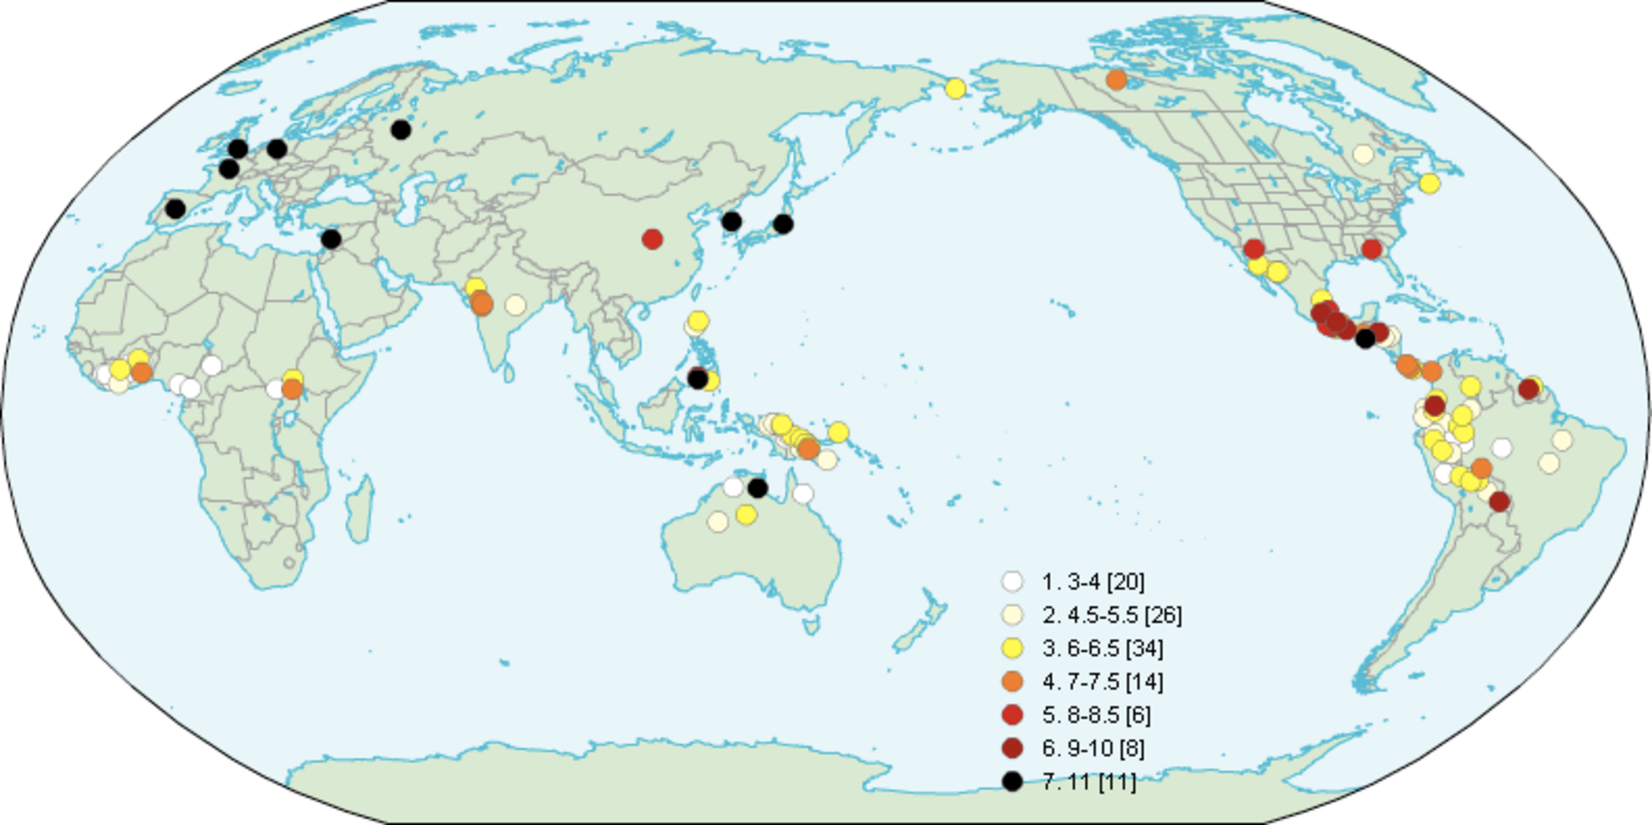
\includegraphics[width=\textwidth]{./intro/figures/number-bcts.pdf}
    \caption[The number of basic colour terms around the world]{The
      number of basic colour terms in languages around the world
      \citep{kay08number}.}
    \label{f:number-bcts}
  \end{center}
\end{figure}

Other systems based on this strategy vary in which dimensions of the
colour domain are relevant for the basic colour terms. The basic
colour system of Hunan\'oo, a language spoken by the Mangyans in the
Philippines, consists of four colour terms: \textit{(ma)biru} (`blackness'),
\textit{(ma)lagti} (`whiteness'), \textit{(ma)rara} (`redness') and \textit{(ma)latuy}
(`greenness'). In this system only the lightness and the red-green
opponent channels are relevant to name colours whereas the yellow-blue
opponent channel is ignored \citep{conklin55hanunoo}.

\subsection{Graded membership strategy}

The fact that each colour category has a focal colour also
implies that other colour samples are worse examples of a particular
colour category. Some languages allow their users to mark how well a
particular sample represents the prototype. In English this marking is
optional and achieved through the adverb \textit{very} and the modifying
\textit{-ish} suffix, for instance in the expression \textit{greenish}. In other
languages, such as Tarahumara, which is an indigenous language spoken
in the North of Mexico, this marking is obligatory. This language has
an elaborate system of modifiers that distinguishes three levels of
membership: \textit{-kame} which could be translated as `very', \textit{-name}
which could be glossed as `somewhat' and \textit{-nanti} for the lowest
degree of membership. An example of how this system is used for the
Turahumara colour category for red: \textit{sit\'a-} is shown in \figref{f:tarahumara} \citep{burgress83tarahumara}.

\begin{figure}[htbp]
  \begin{center}
   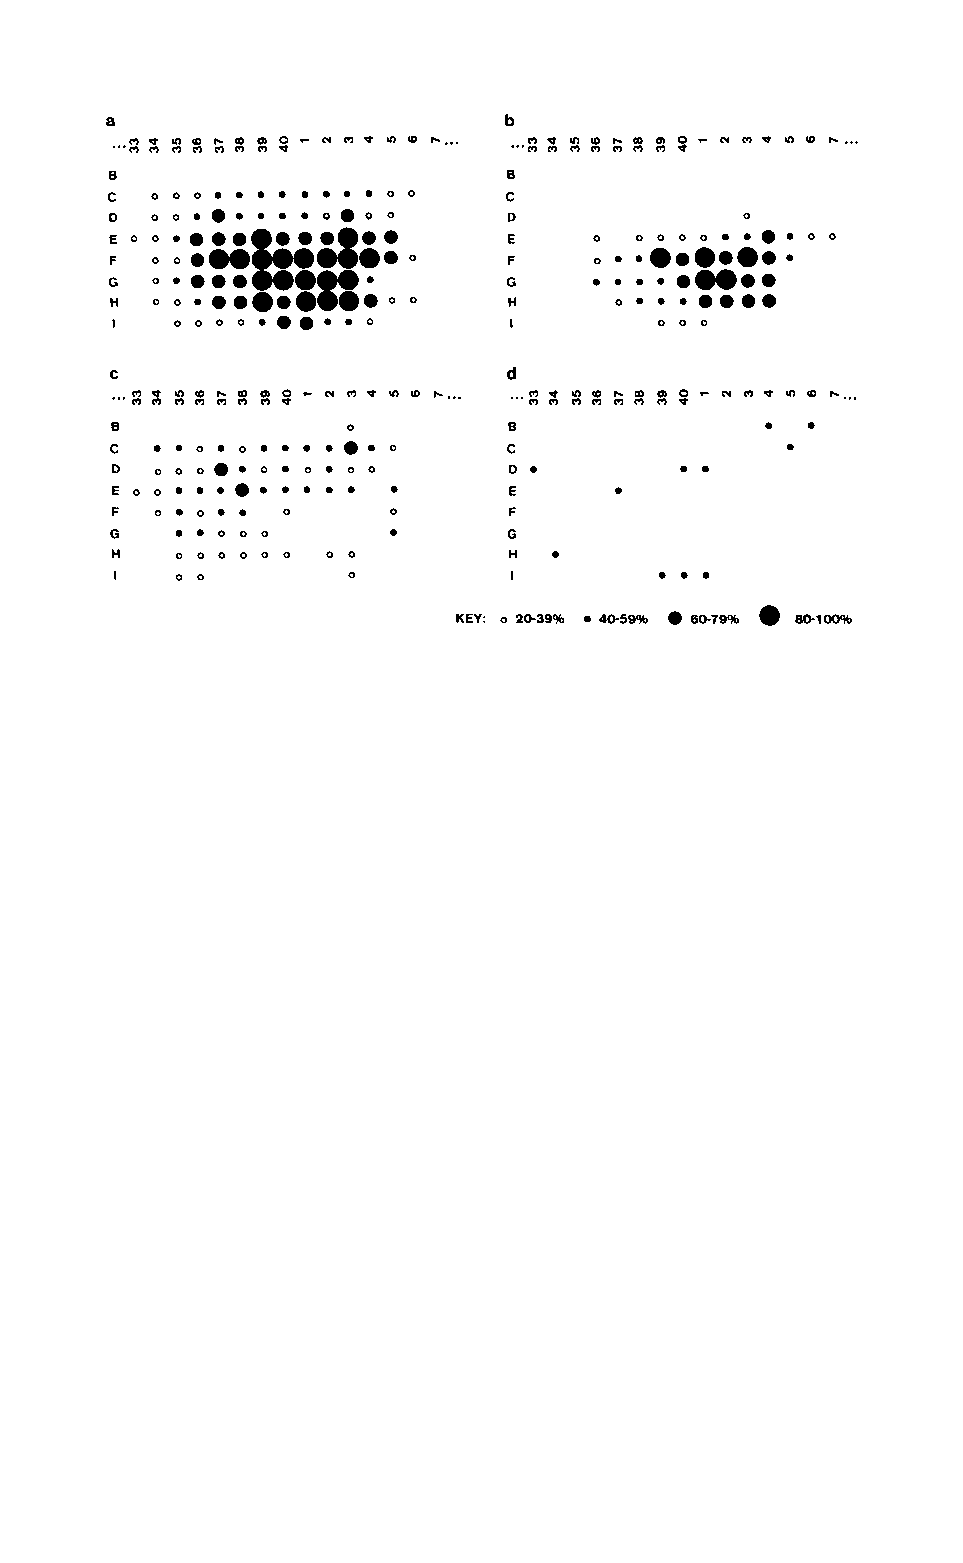
\includegraphics[width=\textwidth]{./intro/figures/tarahumara.pdf}
   \caption[The use of modifiers in Tarahumara]{The use of modifiers
     to express graded membership in Tarahumara shown on an array of
     Munsell chips. The bigger the circle, the more it represents a
     particular colour expression. (a) aggregate of all expressions
     using the \textit{sit\'a} root (b) \textit{sit\'akame} (very red) (c)
     \textit{sit\'aname} (somewhat red) (d) \textit{sit\'ananti} (only slightly
     red). Note how each modifier specifies a region that is further
     removed from the prototypical colour of \textit{sit\'a}. Figure from
     \cite{burgress83tarahumara}.}
    \label{f:tarahumara}
  \end{center}
\end{figure}

\subsection{Compounding strategy}

Some languages also allow users to compound two colour categories into
a new one. Especially to describe a colour sample that is not a good
example of any of the basic colour categories, this might be a very
productive strategy that increases expressivity. An example in English
would be \textit{blue-green}. This compounding can also be modulated by
additional markers, like for example the \mbox{\textit{-ish}} marker as in
\textit{brownish-red} in English.

\cite{safuanova07russian} have collected data on the focal colours of
compounds in Russian. One of their main findings is that in Russian
the order in which colour terms are compounded has an influence on
the resulting focal colour: the second term seems to be more important
in the expression. This is illustrated in the upper left segment of
\figref{f:category-combination}. The colours between \textit{\v
z\"eltyj} (`yellow') and \textit{zel\"enyj} (`green') are for example named:
\textit{zelenovato-\v z\"eltyj} (`greenish-yellow'), \textit{zel\"eno-\v z\"eltyj}
(`green-yellow'), \textit{\v z\"elto-zel\"enyj} (`yellow-green') and \linebreak\textit{\v
z\"eltovato-zel\"enyj} (`yellowish-green') where the suffix \textit{-ato}
acts as a modulator.

\begin{figure}[htbp]
  \begin{center}
   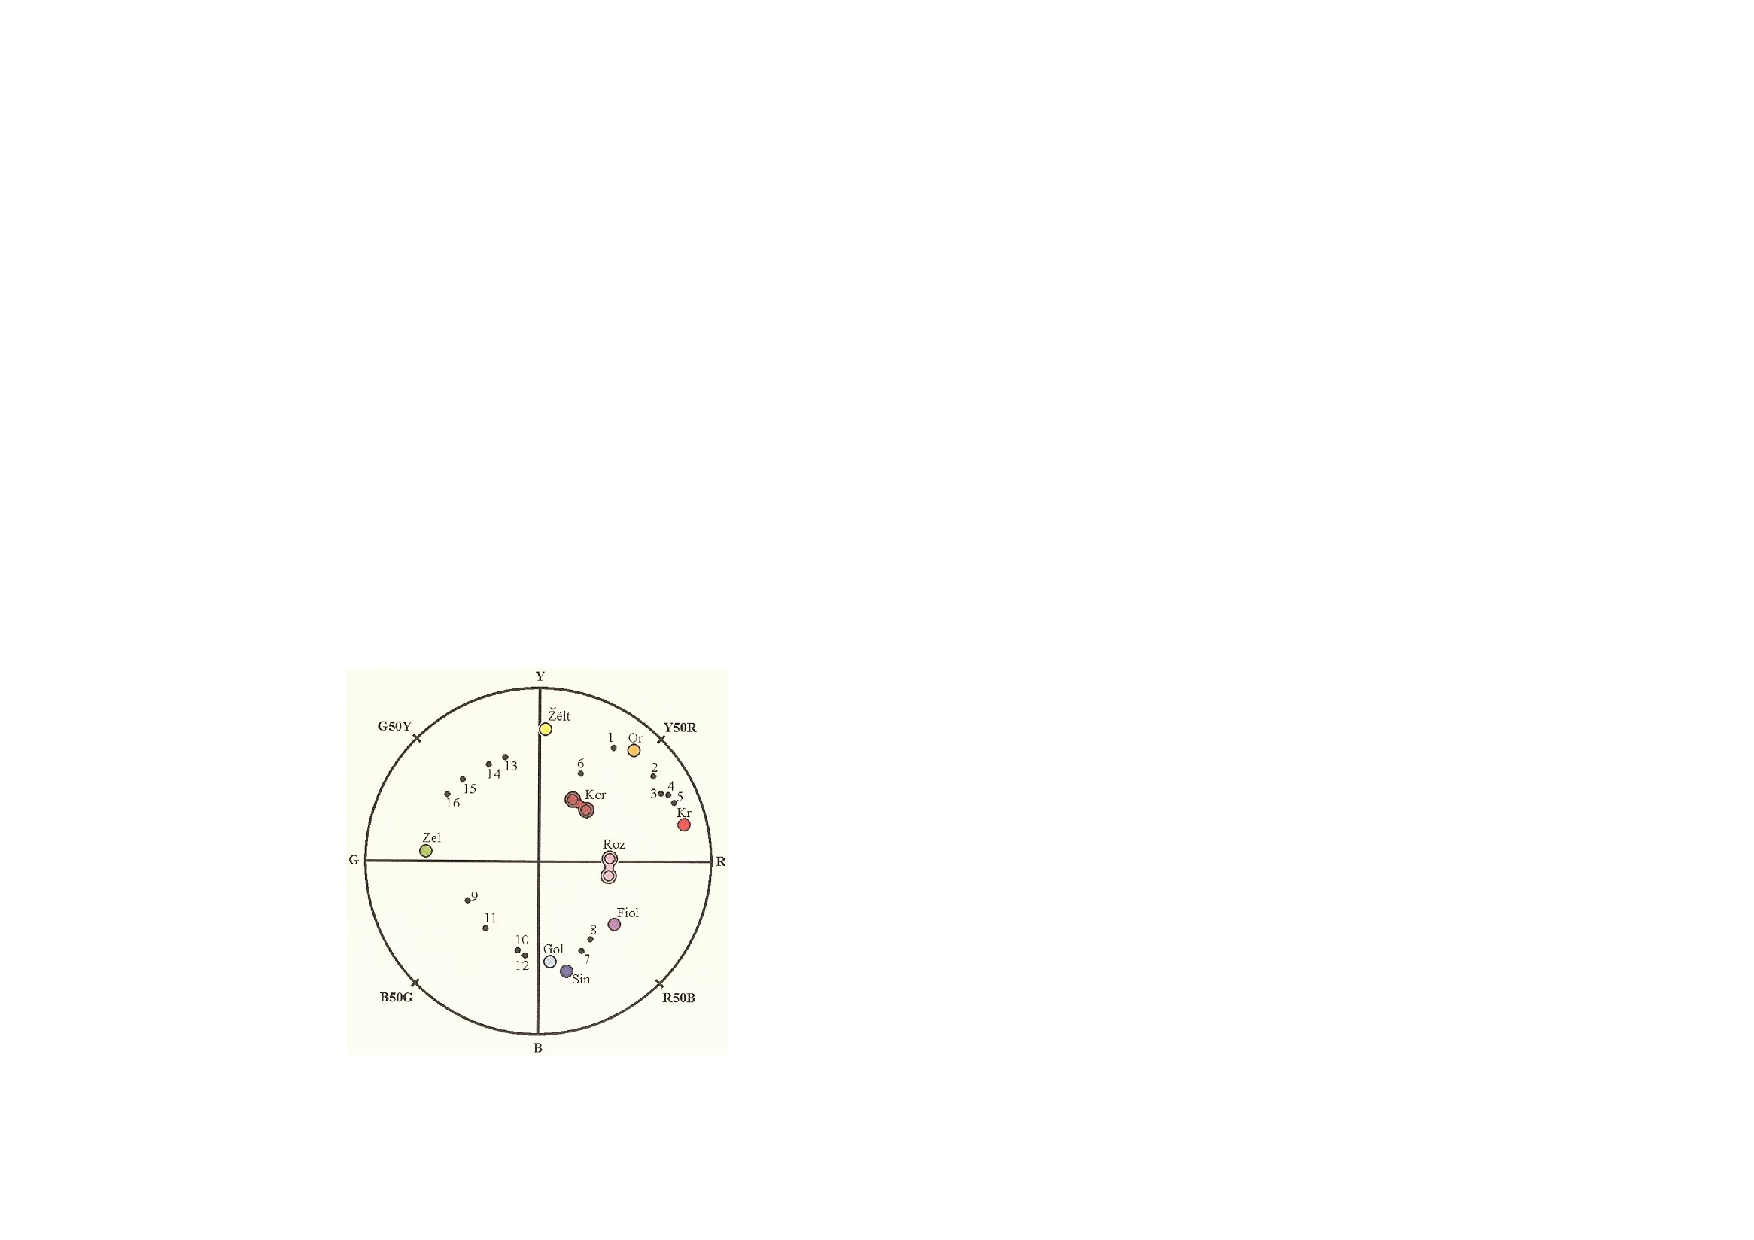
\includegraphics[width=0.6\textwidth]{./intro/figures/category-combination.pdf}
   \caption[Compound chromatic terms in Russian]{Compound chromatic
     terms projected on the hue plane of the NCS colour space. The
     second term in the compound clearly has a bigger impact on the
     resulting focal colour than the first one. The colours between
     \textit{\v z\"eltyj} (`yellow') and \textit{zel\"eno} (`green') are for example
     named: (13) \textit{zelenovato-\v z\"eltyj} (`greenish-yellow'), (14)
     \textit{zel\"eno-\v z\"eltyj} (`green-yellow'), (15) \textit{\v
     z\"elto-zel\"enyj} (`yellow-green') and (16) \textit{\v
     z\"eltovato-zel\"enyj} (`yellowish-green'). Figure from
     \cite{safuanova07russian}.}
    \label{f:category-combination}
  \end{center}
\end{figure}

\subsection{Basic modification strategy}

Similarly, many language systems allow for the use of basic
modifiers which modify some aspects of a colour category. In English
for example, users can modify the brightness and the chromaticity of a
colour category through the use of modifiers (\textit{light} or \textit{dark}
for modifying the brightness and \textit{bright} or \textit{pale} for modifying
the chromaticity). This strategy has been attested for a wide range of
languages, including Vietnamese \citep{alvarado02modifying} and
Chinese \citep{lin01unconstrained}.

Although basic modifiers are quite commonly used, only a few
papers report on the exact transformation that is implied by these
modifiers. One exception is the study by \cite{safuanova07russian} of
the Russian language, in which the authors determined the focal
colours of the modified categories. An example of such an analysis in
the Natural Color Sytem (see Appendix \ref{s:NCS}) is shown in \figref{f:intro-russian-modifiers}. The modifiers \textit{t\"emno-} (`dark') and
\textit{svleto} (`light'), modify the focus of the basic category parallel to
the blackness dimension (W-S). The modifiers \textit{bledno-} (`pale') and
\textit{jarko-} (`bright') shift the chromaticity of the basic colour
category (W-C or S-C) \citep{safuanova07russian}.

\begin{figure}[htpb]
  \centering
  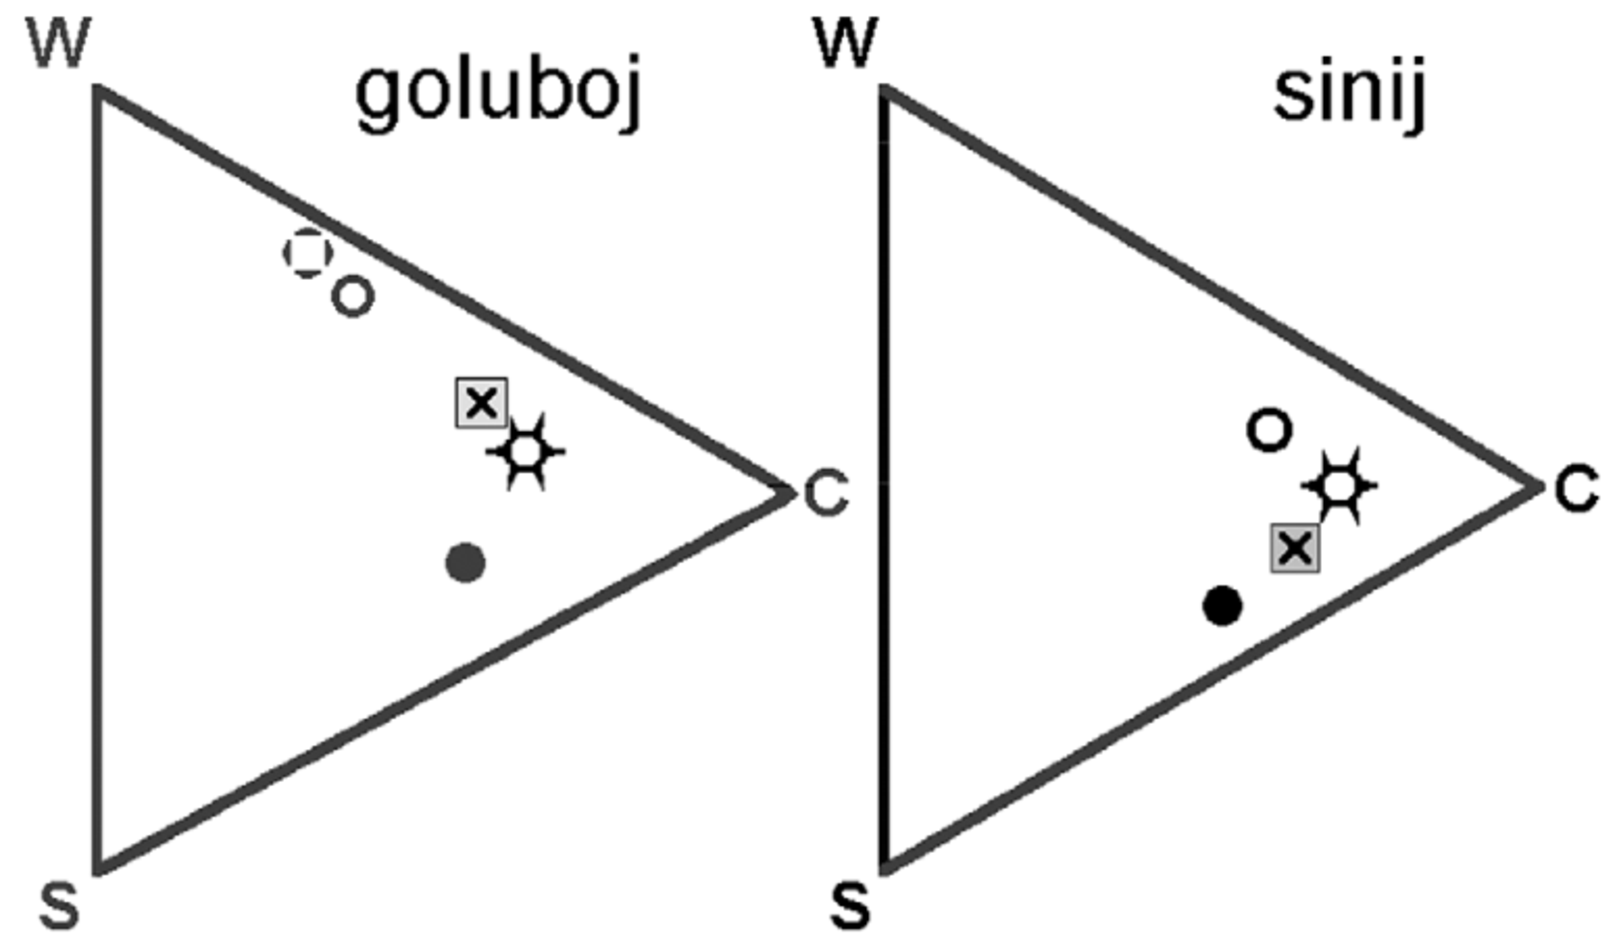
\includegraphics[width=.5\textwidth]{./intro/figures/russian-diagram.pdf}
  \caption[Location of modified basic colour foci in Russian]{Location
    of modified basic colour foci in Russian projected into the NCS
    blackness-chromaticity triangle. \textit{t\"emno-} (`dark', solid
    circle), \textit{jarko-} (`bright', sun), \textit{svetlo-} (`light', open circle) and  \textit{bledno-} (`pale', dashed circle). Figure
    from \cite{paramei05singing}.}
  \label{f:intro-russian-modifiers}
\end{figure}

\subsection{Other strategies}

Another strategy that is often used to name colours, is suggesting
colours by naming an object that is typical for that colour (like for
example \textit{lavender} or \textit{salmon} in English). These object names can
also be used in combination with basic colour terms (like \textit{sky blue}
or \textit{cherry red}). Even though the abundant usage of these terms has
been confirmed in unconstrained naming experiments, like for example
in English and Chinese \citep{lin01unconstrained}, the actual focal
colours of these expressions have yet to be determined. The previous
list of language strategies is not exhaustive, as other strategies to
describe colours exist (for example using comparatives like in \textit{most green}).

\section{Modelling a language strategy}
\is{language strategy!modelling}

Modelling a language strategy starts with the reverse engineering of
the semantic and syntactic templates that allow language users to
conceptualise and express a particular subarea of meaning in
language. A language strategy also includes the operationalisation of
a series of learning operators, which will be discussed later.

In the \textsc{basic colour strategy}, the semantic template defines how
to select the appropriate colour category to describe a colour sample,
for example, the category that is most similar to that sample. The
syntactic template could then define a lexicon in which categories are
associated to terms. These templates can be used in both production
and interpretation.

The performance of the semantic and syntactic templates can be
evaluated in a \textsc{baseline experiment}\is{baseline experiment}. 
In such an experiment, these templates are instantiated
based on a natural language system that is provided by the
experimenter. It allows to model a natural language system and to test
its simulated performance in a benchmark using simulated language
users, or agents.

\subsection{Modelling linguistic interaction}
\label{s:intro-language-games}

In order to model the function of a language strategy, I will use the
language game paradigm \citep{steels96self}. In this paradigm,
language users are modelled as \textsc{agents}\is{agent} and a language community
as a \textsc{population of agents}. These agents constantly engage in
local interactions, or \textsc{language games}\is{language game} in
which they try to achieve \textsc{communicative goals}\is{communicative goal}, like for example drawing the
attention of another agent to one of the objects in a shared
environment or \textsc{context}\is{context}. Achieving these communicative goals is considered to be
the function of a language strategy.

A language game typically involves two agents randomly drawn from the
population. One is assigned the role of the speaker and the other the
role of the hearer. The speaker selects a private communicative goal,
for which it conceptualises a meaning. Using its current linguistic
knowledge it produces an utterance to express this meaning. The hearer
parses this utterance using its own current linguistic knowledge and
interprets the resulting meaning in his own world model. This
interpretation might lead to some actions which should allow the
speaker to verify whether the intended communicative goal was
reached. If this is not the case, the speaker reveals the
communicative goal to the hearer. Both agents update their linguistic
and conceptual knowledge in order to become more successful in future
interactions. All the processes involved in one interaction are
summarised in a \textsc{semiotic cycle}\is{semiotic cycle} which is
shown in \figref{f:intro-semiotic-cycle}
\citep{steels03reentrance}.

\begin{figure}
  \begin{center}
   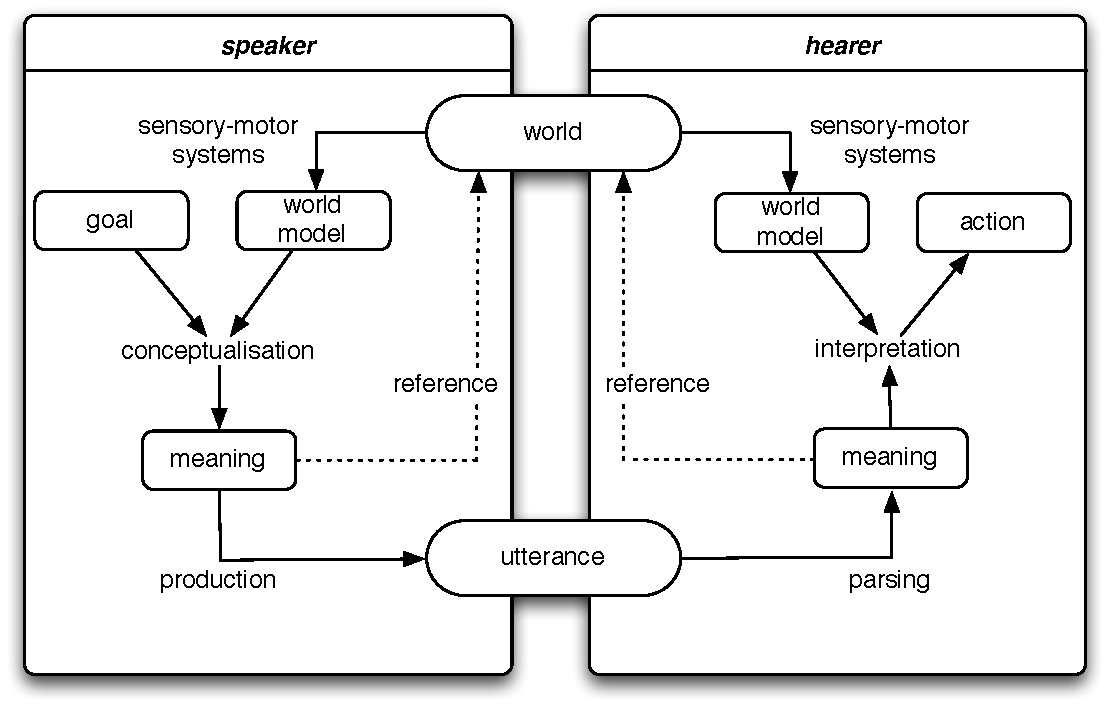
\includegraphics[width=.8\textwidth]{./intro/figures/semiotic-cycle.pdf}
   \caption[The semiotic cycle of a language game]{The semiotic cycle
     of a language game. The speaker selects a communicative goal
     using its own world model, conceptualises a meaning and renders
     an utterance for this meaning. The hearer parses this utterance
     into meaning which is interpreted using its own world model. This
     interpretation might lead to some action, upon which the speaker
     provides feedback (not shown in figure).}
    \label{f:intro-semiotic-cycle}
  \end{center}
\end{figure}

\subsubsection{Language games for colour}
\label{s:language-games-for-colour}

The first language game in which colour could be expressed by the
agents, was the Talking Heads experiment
\citep{steels99talking}. In this experiment contexts consisted
of coloured geometrical figures on a whiteboard which were perceived
by two pan-tilt cameras. Software agents could be embodied in these
cameras. The communicative goal was to draw the attention of the other
agent to one of these figures. The agents could describe several
domains to achieve this goal, including the domain of colour. It soon
became apparent that the domain of colour was rich and complex enough
to be studied in isolation.

This observation led to the development of the \emph{Colour Naming
  Game}\is{language game!Colour Naming Game}\is{Colour Naming
  Game|see{language game}} \citep{steels05coordinating,
  belpaeme05explaining, belpaeme07language, puglisi08cultural,
  baronchelli10modeling} in which agents were restricted to use only
the domain of colour to achieve the communicative goal. The use of
information in other domains, for example spatial relations, was not
allowed. The Colour Naming Game has been devised to study how a
population of agents can form and align its own colour category
systems. In these studies the contexts were based on the random
selection of a number of colour samples from a large set of
colour samples. A colour sample is an abstract representation that
only contains colour information.

In the \emph{Grounded Colour Naming Game}\is{language
game!Grounded Colour Naming Game}\is{Grounded Colour Naming
Game|see{language game}} (see \sectref{s:experiments-grounded}),
embodied agents (ro\-bots) are placed in a closed office environment and
the contexts consisted of toy-like objects that are placed in front of
the agents. Although embodied agents could easily use different
domains to describe the objects in front of them, they are only
allowed to describe the colour information of these objects. In this
language game, the utterances are still restricted to a single term.

I introduce the \emph{Colour Description Game}\is{language
  game!Colour Description Game}\is{Colour Description
  Game|see{language game}} (see Chapters
\ref{s:graded-membership-strategy}--\ref{s:basic-modification-strategy})
in which the restriction of using a single colour term to describe the
colour of an object is lifted.

\subsubsection{Background assumptions}

The language paradigm focusses on the functional and evolutionary
aspect of languages, but this can only be achieved by making some
assumptions. It is assumed that agents are capable of giving joint
attention \citep{tomasello95jointattention}, constructing world
models, taking turns, being cooperative\footnote{\cite{wang08self}
  show that uncooperative agents can also bootstrap a language under
  certain conditions.}, and so on. These assumptions are each
interesting and far from trivial research topics by
themselves. Although it is clear that these processes are
prerequisites for studies in the language game paradigm, they are not
in the main focus of this paradigm.

\section{Self-organisation of language systems}

A language system is not a static system, but rather a living system
that is constantly evolving. In the self-organisation of language systems
based on the basic colour strategy, language systems are expanded by
the introduction of new colour categories. By studying a wide range of
contemporary language systems for colour, some researchers have even
proposed a universal evolutionary order by which colour categories are
introduced to a language \citep{berlin69basic}.

% todo: meer uitleg

\section{Modelling the self-organisation of language systems}

In order to model the self-organisation of language systems\is{language system!self-organisation of}, 
the implementation of a language strategy needs
to be extended with a series of learning operators that specify:

\begin{enumerate}
\item how a language user can acquire a language system from other
  language users using \textsc{adoption operators}\is{learning operators!adoption operator}
\item how language users can update their knowledge of the language
  system after a linguistic interaction using \textsc{alignment
    operators}\is{learning operators!alignment operator}
\item how a language user can expand a language system using
  \textsc{invention operators}\is{learning operators!invention operator}
\end{enumerate}

For the basic colour strategy, the adoption operator allows a user to
adopt a new colour category and its associated colour term when a new
unknown term is encountered. The invention operators allow users to
introduce new colour terms that are associated to new colour
categories to the language system. Finally, the alignment operator
specifies that agents should update their colour categories to better
represent the topic when the linguistic interaction was successful.

An \textsc{acquisition experiment}\is{acquisition experiment} could be implemented in which the
adoption and alignment operators of a language strategy are
tested. Such an experiment involves two agents in which one needs to
acquire a predefined language system from another agent. By comparing
the performance of the agent that is acquiring the language system to
the performance in the baseline experiment, the performance of the
adoption and alignment operators can be evaluated.

The final step would be a \textsc{formation experiment}\is{formation experiment} in which a
population of agents needs to construct its own language system from
scratch. Such an experiment checks the performance of the invention
operators by comparing the performance of the population of agents in
this experiment to the baseline performance.

\subsection{Language as a complex adaptive system}
 
Within the language game paradigm, a language system is considered to
be a complex adaptive system \citep{steels00language}. It is shaped
and reshaped by its users to suit their needs, even over the course of
a single dialogue \citep{garrod94conversation}, in order to become
more successful in communication while minimising cognitive effort. No
single user has a complete view of the language and no user can
control the linguistic behaviour of the complete group. Instead,
language is a self-organising system that emerges through local
interactions or language games.

\section{Evolution of language strategies}
\is{language strategy!evolution}

If one takes a historical perspective on language, one can also
detect shifts in dominance from one language strategy to another. In
the evolution of the basic colour terms in English an interesting
meaning shift occurred: at their Indo-European root most colour terms
had primarily a brightness meaning sense. Around the transition from
Old to Middle English the hue meaning sense of all basic colour terms became
more dominant than the original brightness sense
\citep{casson97shift}. Both meaning senses could be thought of as
different variations of the basic colour strategy.

This is illustrated in \figref{f:history-yellow} in which the
history of the term \textit{yellow} is shown. In Indo-European its
syntactic form was \textit{ghel} which was primarily used to refer to the
shining (of yellow metals). In Old English the term \textit{geolo} acquired
a hue sense and could be used to refer to the colour of some silk
cloth. In the transition to Middle English \textit{yelou} the hue sense
became the more dominant one and the term could also be used to refer
to for example yolk and ripe corn, although it could still be used to
refer to gold. The same is true for all other basic colour terms. Most
interestingly, all colour terms that were introduced to English after
this shift, like for example \textit{orange}, never had a brightness sense
but only a hue sense \citep{casson97shift}. Similar meaning shifts
have been reported in a wide range of languages
\citep{maclaury92brightness}.

\begin{figure}
  \begin{center}
   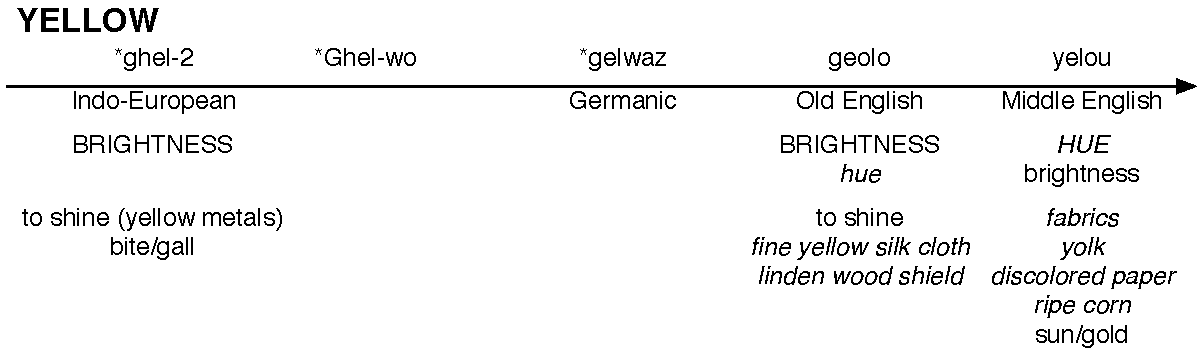
\includegraphics[width=.8\textwidth]{./intro/figures/history-yellow.pdf}
   \caption[The evolution of the term \textit{yellow} in English]{The
     evolution of the term \textit{yellow} in English. Like almost all
     other basic colour terms, its meaning shifted from brightness to
     hue around the transition from Old English to Middle
     English \citep{casson97shift}.}
    \label{f:history-yellow}
  \end{center}
\end{figure}

\section{Modelling evolution of language strategies}

Given the observed evolution and selection at both the level of
language strategies and the level of linguistic items that make up a
particular language system, I explore the hypothesis that linguistic
agents need explicit representations of language strategies which they
use to keep track of how successful a particular strategy has been in
communication. These explicit representations allow me to introduce an
additional layer of selection at the level of language strategies.

\section{Structure of this book}

\chapref{s:formalisms} will introduce the formalisms that will be 
used to model language strategies and language systems.

\partref{s:language-strats} of this book focusses on the
reconstruction of the general semantic and syntactic structures that
allow me to run baseline experiments for several of the language
strategies identified in this chapter: the basic colour strategy, the
graded membership strategy, the compounding strategy and the
basic modification strategy.

In \partref{s:evolution-of-language-systems}, I will focus on the
self-organisation of language systems that are based on one language strategy,
namely the basic colour strategy, by introducing its adoption,
alignment and invention operators. This will allow me to study the
impact of embodiment on the performance of these operators. I will
also show results of related experiments on language systems that are
realisations of this strategy.

In \partref{s:evolution-of-language-strategies}, I
will present a model that allows to study the evolution of language
strategies based on linguistic selection. I will start by introducing
two variants of the basic colour category and show an experiment that
models the meaning shift as documented for the history of basic colour
terms. I will also explore the origins of language strategies based on
a combinatorial search process.

The concluding \partref{s:conclusion} will give an overview of
the main results that have been achieved in this book and will
outline some directions for future research.
